\documentclass[final]{article}

% if you need to pass options to natbib, use, e.g.:
% \PassOptionsToPackage{numbers, compress}{natbib}
% before loading nips_2017
%
% to avoid loading the natbib package, add option nonatbib:
% \usepackage[nonatbib]{nips_2017}

\usepackage{nips_2017}

% to compile a camera-ready version, add the [final] option, e.g.:
% \usepackage[final]{nips_2017}

\usepackage[utf8]{inputenc} % allow utf-8 input
\usepackage[T1]{fontenc}    % use 8-bit T1 fonts
\usepackage{hyperref}       % hyperlinks
\usepackage{url}            % simple URL typesetting
\usepackage{booktabs}       % professional-quality tables
\usepackage{amsfonts}       % blackboard math symbols
\usepackage{nicefrac}       % compact symbols for 1/2, etc.
\usepackage{microtype}      % microtypography

% \usepackage{lmodern}

\usepackage{graphicx}
\usepackage{caption}
\usepackage{subcaption}
\usepackage{tikz}
\usepackage{float}
\usetikzlibrary{shapes, arrows}

\title{Formatting instructions for NIPS 2017}

% The \author macro works with any number of authors. There are two
% commands used to separate the names and addresses of multiple
% authors: \And and \AND.
%
% Using \And between authors leaves it to LaTeX to determine where to
% break the lines. Using \AND forces a line break at that point. So,
% if LaTeX puts 3 of 4 authors names on the first line, and the last
% on the second line, try using \AND instead of \And before the third
% author name.

\author{
  Forest Kobayashi \\
  Department of Mathematics\\
  Harvey Mudd College\\
  Claremont, CA 91711 \\
  \texttt{fkobayash@hmc.edu} \\
  %% examples of more authors
  \And
  Jacky Lee \\
  Department of Mathematics\\
  Department of Computer Science \\
  Harvey Mudd College \\
  Claremont, CA 91711 \\
  \texttt{jaclee@hmc.edu}
}

\begin{document}
% \nipsfinalcopy is no longer used

\maketitle

\begin{abstract}
  Stock data is very difficult to analyze using classical methods, in
  large part due to heavy involvement of humans in stock pricing. In
  this paper, we examine a new approach to analyzing time-series stock
  data, particularly in the context of grouping correlated stocks.
\end{abstract}

\section{Introduction}
Here is a rough table of contents for our paper, so that the reader
has a rough idea of where we'll be going:
\begin{enumerate}
  \item Motivation (challenges to modelling stock data)
  \item Long-term goal for the model / ideal model architecture
  \item Classification
  \item Findings
  \item Conclusion
\end{enumerate}

\section{Background}
There are many reasons why predicting stock prices is difficult, but
for our model today, we will focus on just two:
\begin{enumerate}
  \item The behavior of a given stock is influenced by hundreds of
    hidden variables --- e.g., the current state of geopolitics,
    governmental fiscal policies (for instance, the US Treasury
    interest rate), the performance of stocks in various other
    markets, etc. Hence, the price of a stock at any given moment is
    an emergent phenomenon, influenced by many small movements of
    markets around the world. Further, these connections themselves
    are in a constant state of flux --- as the market evolves,
    technology improves, and policies are rewritten, the weight each
    of these variables has in influencing pricing will wax and wane.
  \item With the exception of some forms of algo trading, most trading
    strategies are being created and implemented by humans. That is,
    often humans are the ones who perform analysis of market
    information, and make decisions based off the findings. But humans
    are not naturally predisposed to rigorous quantitative analysis,
    and hence markets do not always behave rationally. As an example,
    consider \texttt{Bitcoin}.\footnote{Citation: Gary Evans} Thus,
    an accurate financial model will need to have some method of
    predicting human psychology.
\end{enumerate}

Using modern machine learning techniques, it is possible to control
for some effects of (2) by using previous stock data. However,
less work has been done to model the effects of (1). So, for today's
model, we will focus on methods of preprocessing time series stock
data so as to control for some of the effects of (1).

% Stock prices can be influenced by many factors such as other stock
% prices, anticipation of capital gains or losses, global politics,
% earnings reports, and etc. These factors may each have a different
% weighting on the stock depending on time and which stock is being
% analyzed in question. For example, earnings reports might have
% significantly more impact on stock prices immediately after release as
% opposed to two months after the report comes out. Another example
% would be that global politics might influence the stock price of
% \textbf{LMT} (Lockheed Martin), an aerospace and defense company, more
% than the stock price of \textbf{BKC} (Burger King), a fast food
% restaurant chain.

% Ultimately, humans are the ones who choose to buy, sell, or short
% these stocks based on some analysis, usually not completely
% comprehensive, of the factors they observe. Since humans are often
% unaware or unable to analyze all these competing factors at once,
% their decisions are often unpredictable or at least very difficult to
% predict. As such, predicting the price of stocks by modeling these
% interactions between stock price factors and humans is difficult and
% unwise. Therefore, we have decided to perform stock analysis by only
% analyzing past stock trends. This approach, although loses out on a
% lot of information, is computationally less demanding and easier to
% find data for performing analysis.


\section{The Model}

\subsection{Goals}
Our ultimate goal is to be able to use past stock data to train our
model. Then given some stock trend data for some stock, use our model
to predict the upcoming trends and return a vector of decisions. An
example of the output is shown below.

\[
  \mathbf{y} = \Bigl<P_{buy}(\mathbf{x}), P_{sell}(\mathbf{x}),
  P_{short}(\mathbf{x}), P_{nothing}(\mathbf{x})\Bigr>
\]

Here, $P_{buy}(\mathbf{x})$ represents how confident the model is in
recommending the user to buy the stock. Similarly,
$P_{sell}(\mathbf{x})$ represents selling the stock,
$P_{short}(\mathbf{x})$ represents shorting the stock, and
$P_{nothing}(\mathbf{x})$ represents doing nothing. All these
probabilities should sum to 1.

In order to reach this sort of conclusion, we want our model to
compensate for the effects of (1) in a clever way. In traditional
stock trading practices, there are a few guidelines that are used for
similar determinations:
\begin{enumerate}
  \item Someimtes industries follow trends together. For instance, if
    we see a price drop in one oil stock, we might expect to see drops
    in other oil stocks.
  \item When interest rates go up, yield-bearing financial assests
    increase in value, while the value of equity stocks might
    decrease.
  \item If an earnings report reveals that a stock overestimated its
    expected profits, the value of the stock will decrease.
  \item In times of high uncertainty, money might be pulled out of
    equity assets and moved to yield-bearing financial assets. Hence,
    stock prices might go down.
  \item Bad PR can result in a temporary dip in stock pricing.
\end{enumerate}

These are external factors that cannot be determined purely from the
stock data itself. Often, most of this information comes from news
outlets, press releases, and other media-sharing forums. So, we need
our model to perform the following:
\begin{enumerate}
  \item Scrape real-time text data from news websites, financial
    websites, and (possibly) academic journals in the case that we're
    looking at something like a technology stock.
  \item Perform some sort of Natural Language Processing and Sentiment
    Analysis to determine how this information might affect the market
    if / when it becomes widely publicized.
  \item Somehow combine this information with time-series stock data
    to make a prediction of how the market might behave in the short
    and long term.
  \item Make a trading decision based on this information.
\end{enumerate}
We propose the following prototype model.
\subsection{Prototype Architecture}
\begin{figure}[H]
  \centering
    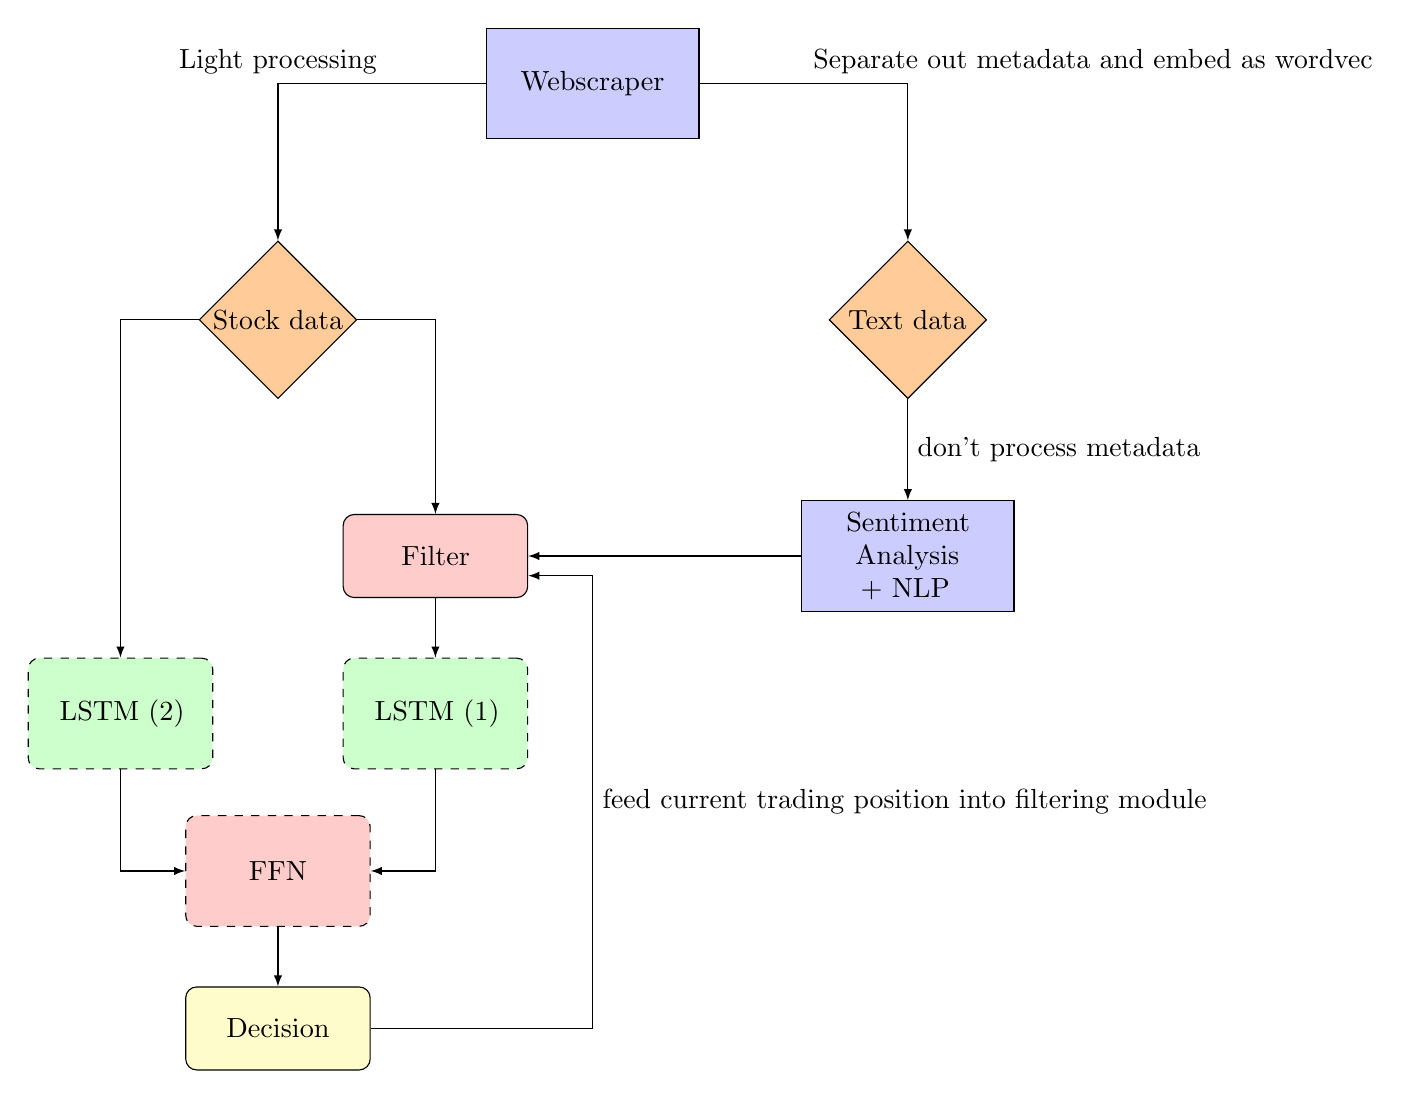
\begin{tikzpicture}[node distance = 2cm, auto]
      \tikzstyle{data} = [
        diamond,
        draw,
        fill=orange!40,
        text width = 5em,
        text badly centered,
        node distance = 3cm,
        inner sep = 0pt
      ]

      \tikzstyle{code} = [
        rectangle,
        draw,
        fill=blue!20,
        text width=7em,
        text centered,
        minimum height=4em
      ]

      \tikzstyle{network} = [
        rectangle,
        draw,
        dashed,
        fill=green!20,
        text width = 6em,
        text centered,
        rounded corners,
        minimum height = 4em
      ]

      \tikzstyle{feedforward} = [
        rectangle,
        draw,
        dashed,
        fill=red!20,
        text width = 6em,
        text centered,
        rounded corners,
        minimum height = 4em
      ]

      \tikzstyle{filter} = [
        draw,
        rectangle,
        fill=red!20,
        text width = 6em,
        text centered,
        minimum height=3em,
        rounded corners
      ]

      \tikzstyle{decision} = [
        draw,
        rectangle,
        fill=yellow!20,
        text width = 6em,
        text centered,
        minimum height=3em,
        rounded corners
      ]

      \node[code] (webscraper) at (0,6) {Webscraper};
      \node[data] (time series) at (-4,3) {Stock data};
      \node[data] (text) at (4,3) {Text data};
      \node[code] (processer) at (4,0) {Sentiment Analysis + NLP};
      \node[filter] (filter) at (-2,0) {Filter};
      \node[network] (lstm1) at (-2,-2) {LSTM (1)};
      \node[network] (lstm2) at (-6,-2) {LSTM (2)};
      \node[feedforward] (feedforward) at (-4,-4) {FFN};

      \node[decision] (decision) at (-4,-6) {Decision};

      \draw[-latex] (webscraper) -| (time series) node[midway, above]
      {Light processing};
      \draw[-latex] (webscraper) -| (text) node[near start, above right]
      {Separate out metadata and embed as wordvec};
      \draw[-latex] (text) -- (processer) node[midway, right] {don't
        process metadata};
      \draw[-latex] (time series) -| (filter);
      \draw[-latex] (filter) -- (lstm1);
      \draw[-latex] (processer) -- (filter);
      \draw[-latex] (time series) -| (lstm2);
      \draw[-latex] (lstm2) |- (feedforward);
      \draw[-latex] (lstm1) |- (feedforward);
      \draw[-latex] (feedforward) -- (decision);
      \draw (decision) -- (0,-6) -- (0,-.25) node[midway, right] {feed
      current trading position into filtering module};
      \draw[-latex] (0,-.25) -- (-.82,-.25) node[midway, right] {};
    \end{tikzpicture}
  \caption{Model overview}
  \label{fig:goal}
\end{figure}

\section{Classification}
Using LSTMs to predict stock pricing is, for the most part, a solved
problem. Implementations and hyperparameters may differ, of course,
but underneath, the structure of the model is largely the same. Hence,
we decided to focus our work on augmenting the filtering stage shown
above. We were particularly interested in finding new representations
of market trends that we could feed into the network.

\section{Methods}

\subsection{Data Scraping}
We gathered intraday data for ten different stocks using the Alpha Vantage API
(\url{https://github.com/RomelTorres/alpha_vantage}). The ten stocks were
randomly selected from the stocks in the S\&P500. A portion of the data for one
stock is shown below.

\begin{verbatim}
                     1. open  2. high   3. low   4. close  5. volume
date
2018-05-08 09:30:00  1058.54  1058.54  1055.00  1055.1600    26407.0
2018-05-08 09:31:00  1054.99  1058.16  1054.99  1056.9248     6384.0
2018-05-08 09:32:00  1057.41  1058.95  1057.41  1058.5700     7160.0
2018-05-08 09:33:00  1058.30  1058.64  1056.93  1058.6400     6448.0
2018-05-08 09:34:00  1058.80  1060.00  1058.50  1059.9600     5548.0
\end{verbatim}

For each stock, we computed the arithmetic mean of the high and low as a
heuristic that summarized the price of the stock in that minute.

\subsection{Polynomial Fitting on Windowed Data}

We then analyzed this time series data by focusing in on windows of 20 minutes
and fitting a cubic polynomial then extracting the constant, linear, and
quadratic coefficients. Each consecutive window was only shifted by 2 minutes
so consecutive windows would have significant overlap. Our reasoning was that
this would make the coefficients be more similar and enable us to have smoother
data.

\begin{figure}[H]
  \centering
  \begin{subfigure}{.3\textwidth}
    \centering
    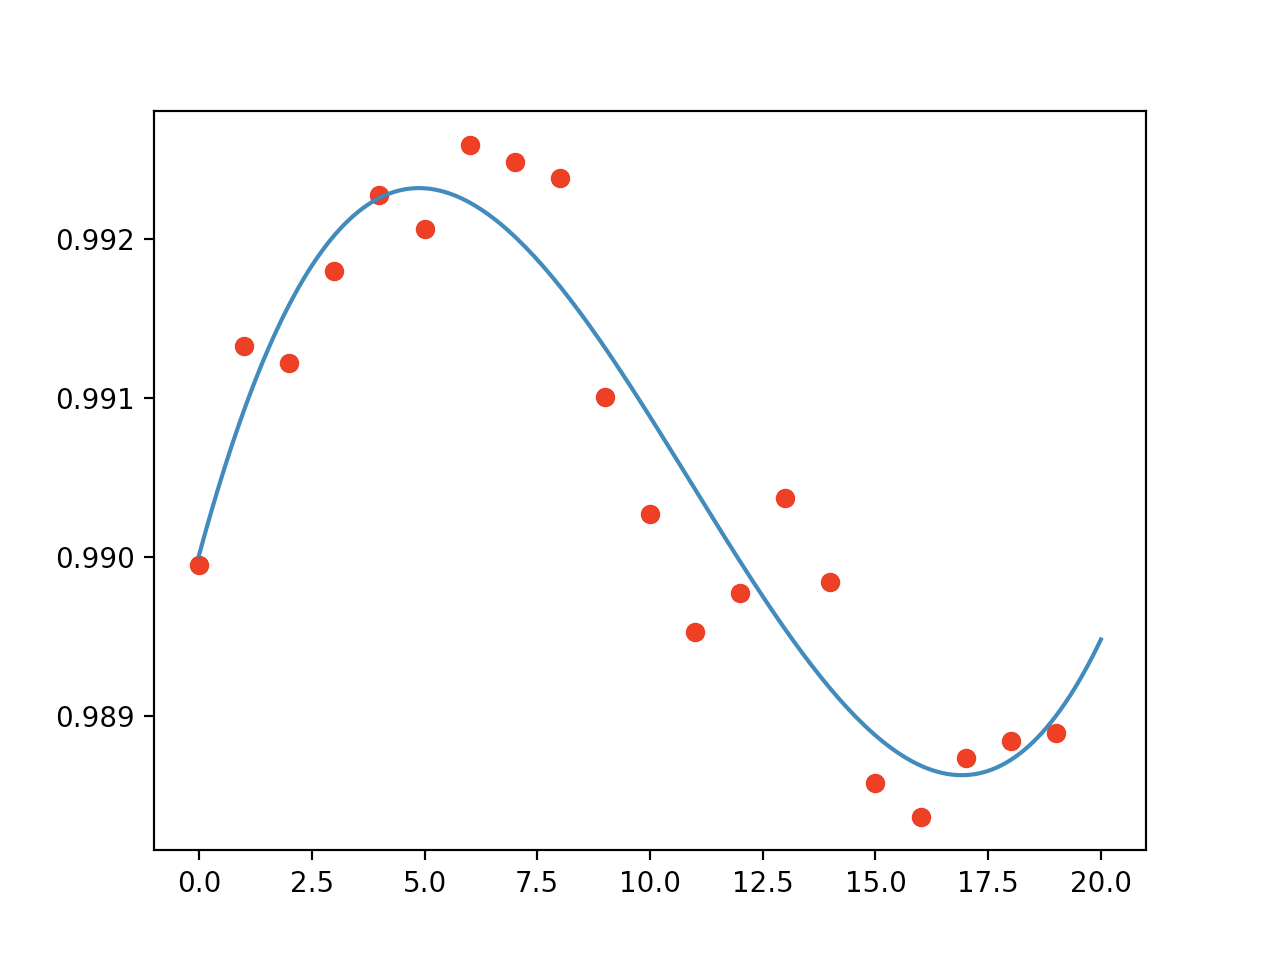
\includegraphics[width=\linewidth]{img/sliding1}
  \end{subfigure}
  \begin{subfigure}{.3\textwidth}
    \centering
    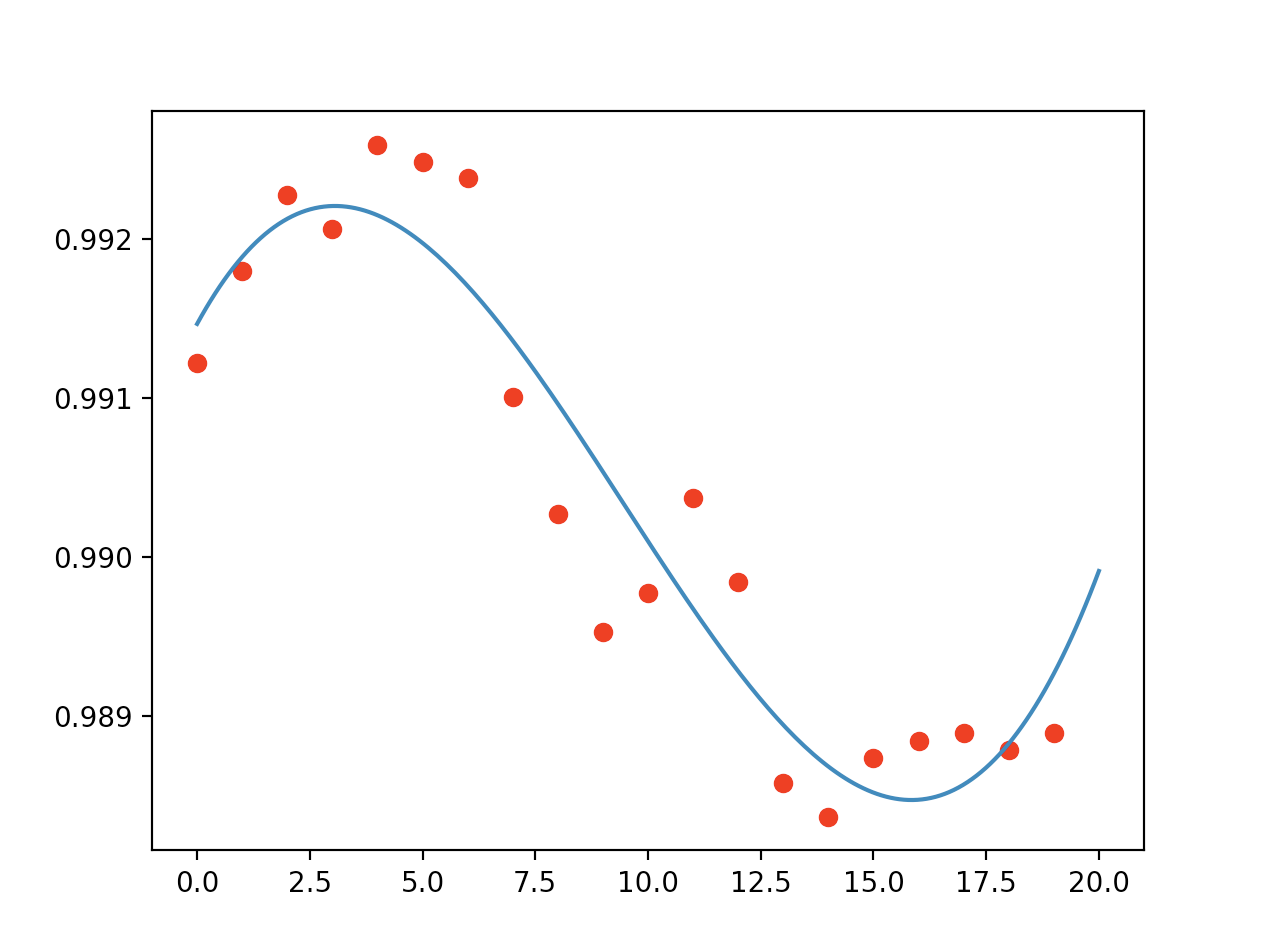
\includegraphics[width=\linewidth]{img/sliding2}
  \end{subfigure}
  \begin{subfigure}{.3\textwidth}
    \centering
    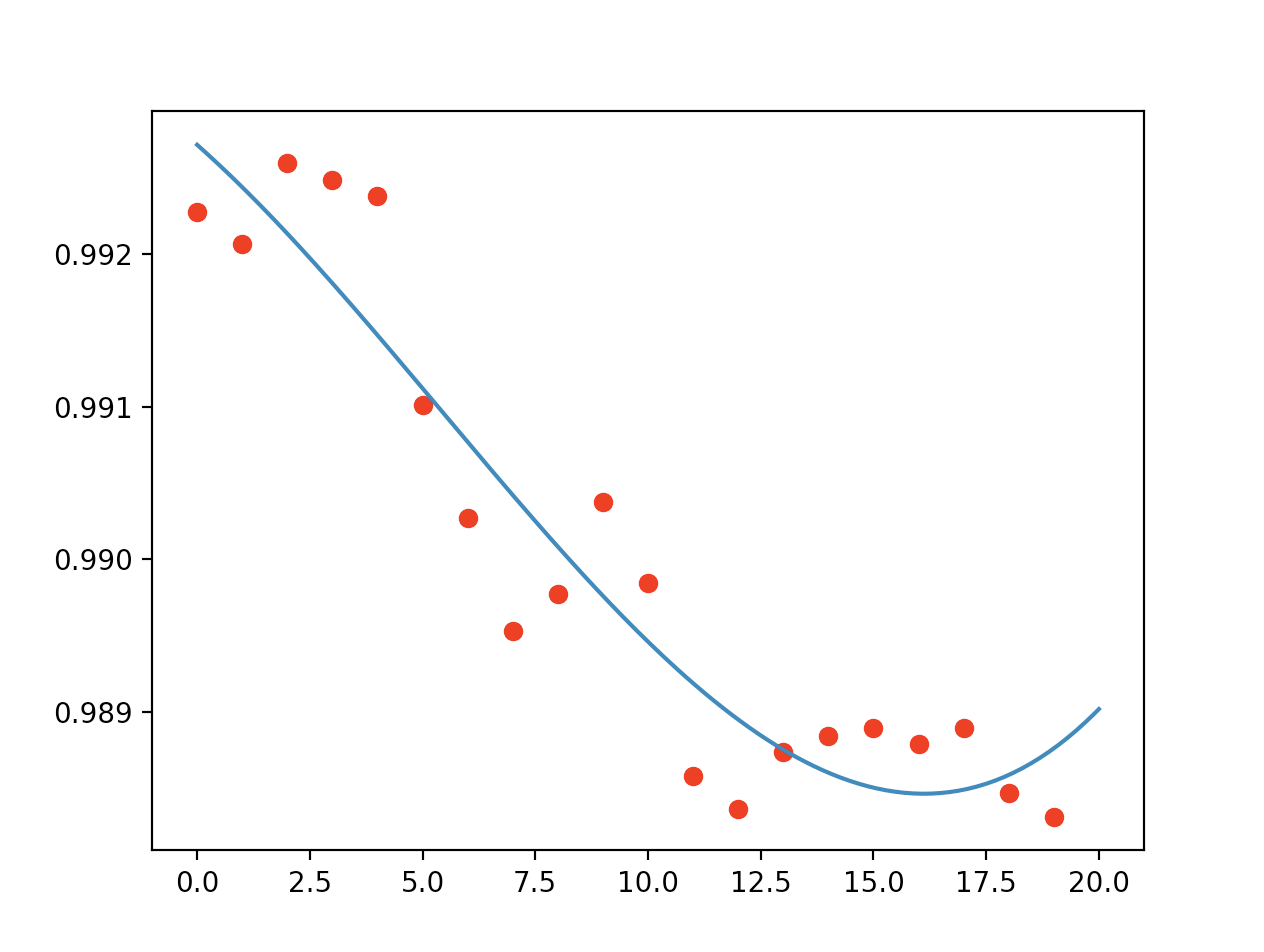
\includegraphics[width=\linewidth]{img/sliding3}
  \end{subfigure}
  \caption{Sliding windows of data fitted with polynomials}
  \label{fig:sliding}
\end{figure}

\subsection{Visualizing the Coefficients}

We then plotted the coefficients of our polynomial fits in $\mathbb{R}^3$
to visualize our data.

\begin{figure}[H]
  \centering
  \begin{subfigure}{.45\textwidth}
    \centering
    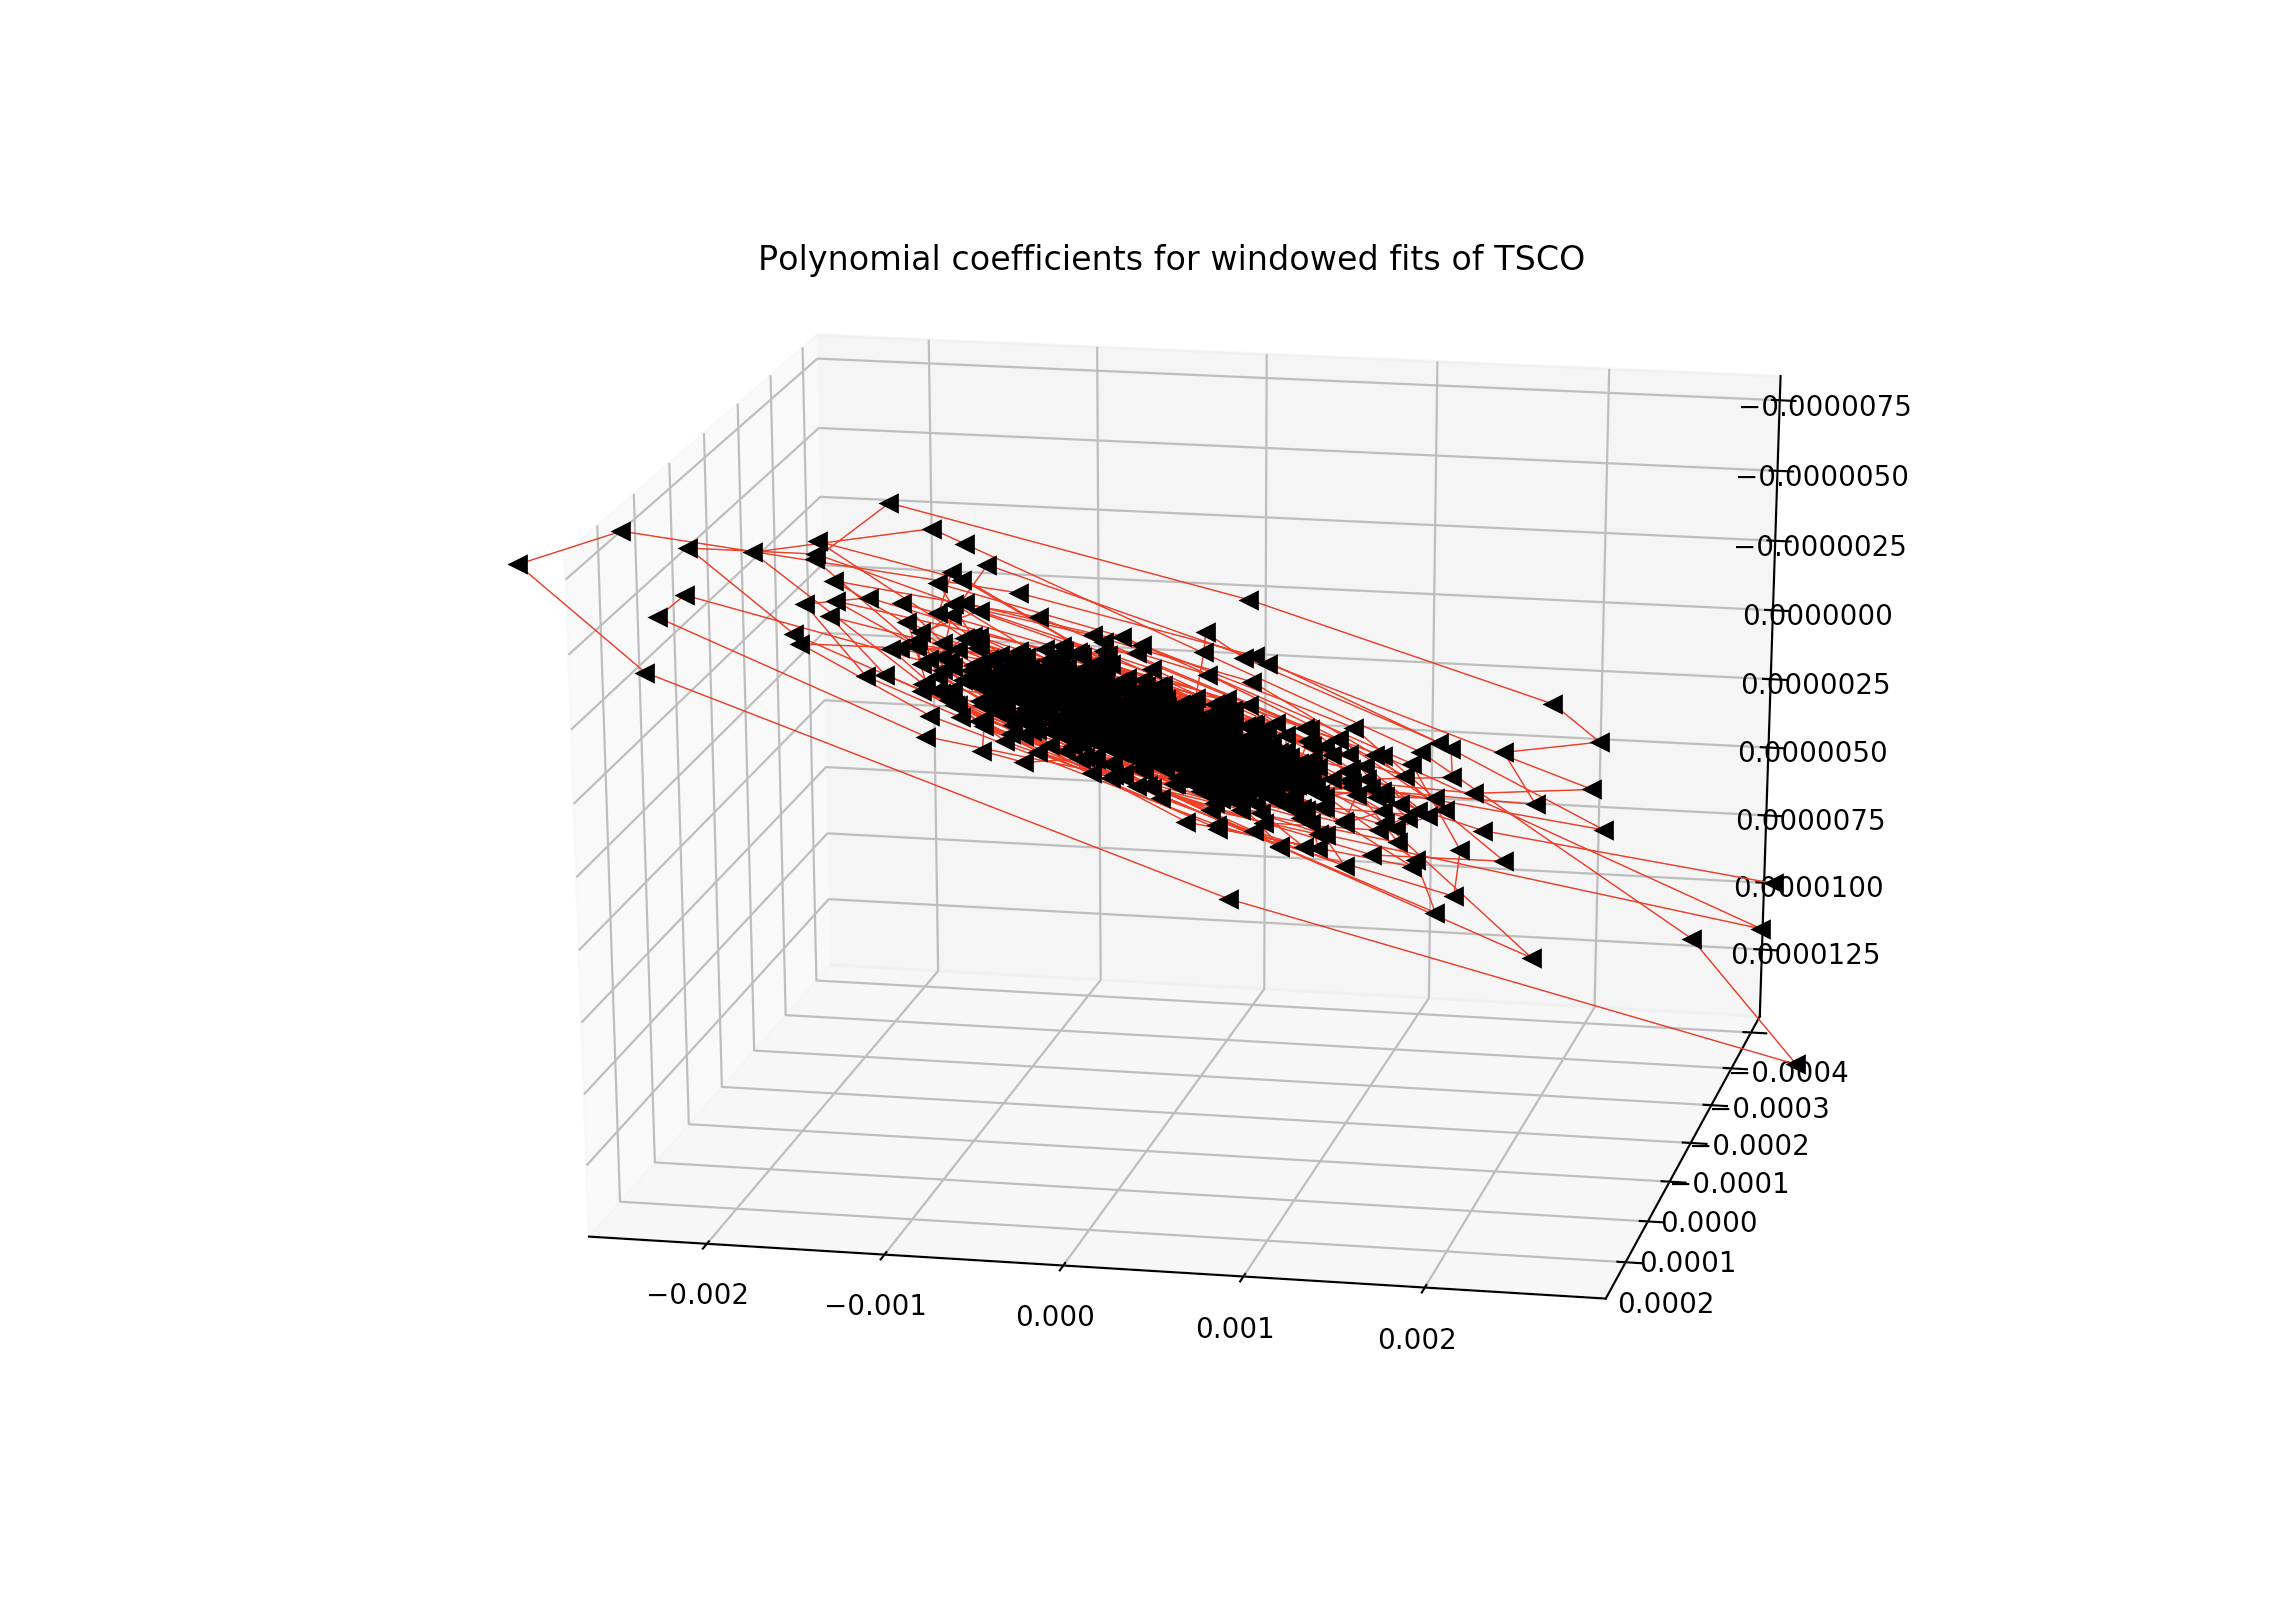
\includegraphics[width=\linewidth]{img/coeff1}
  \end{subfigure}
  \begin{subfigure}{.45\textwidth}
    \centering
    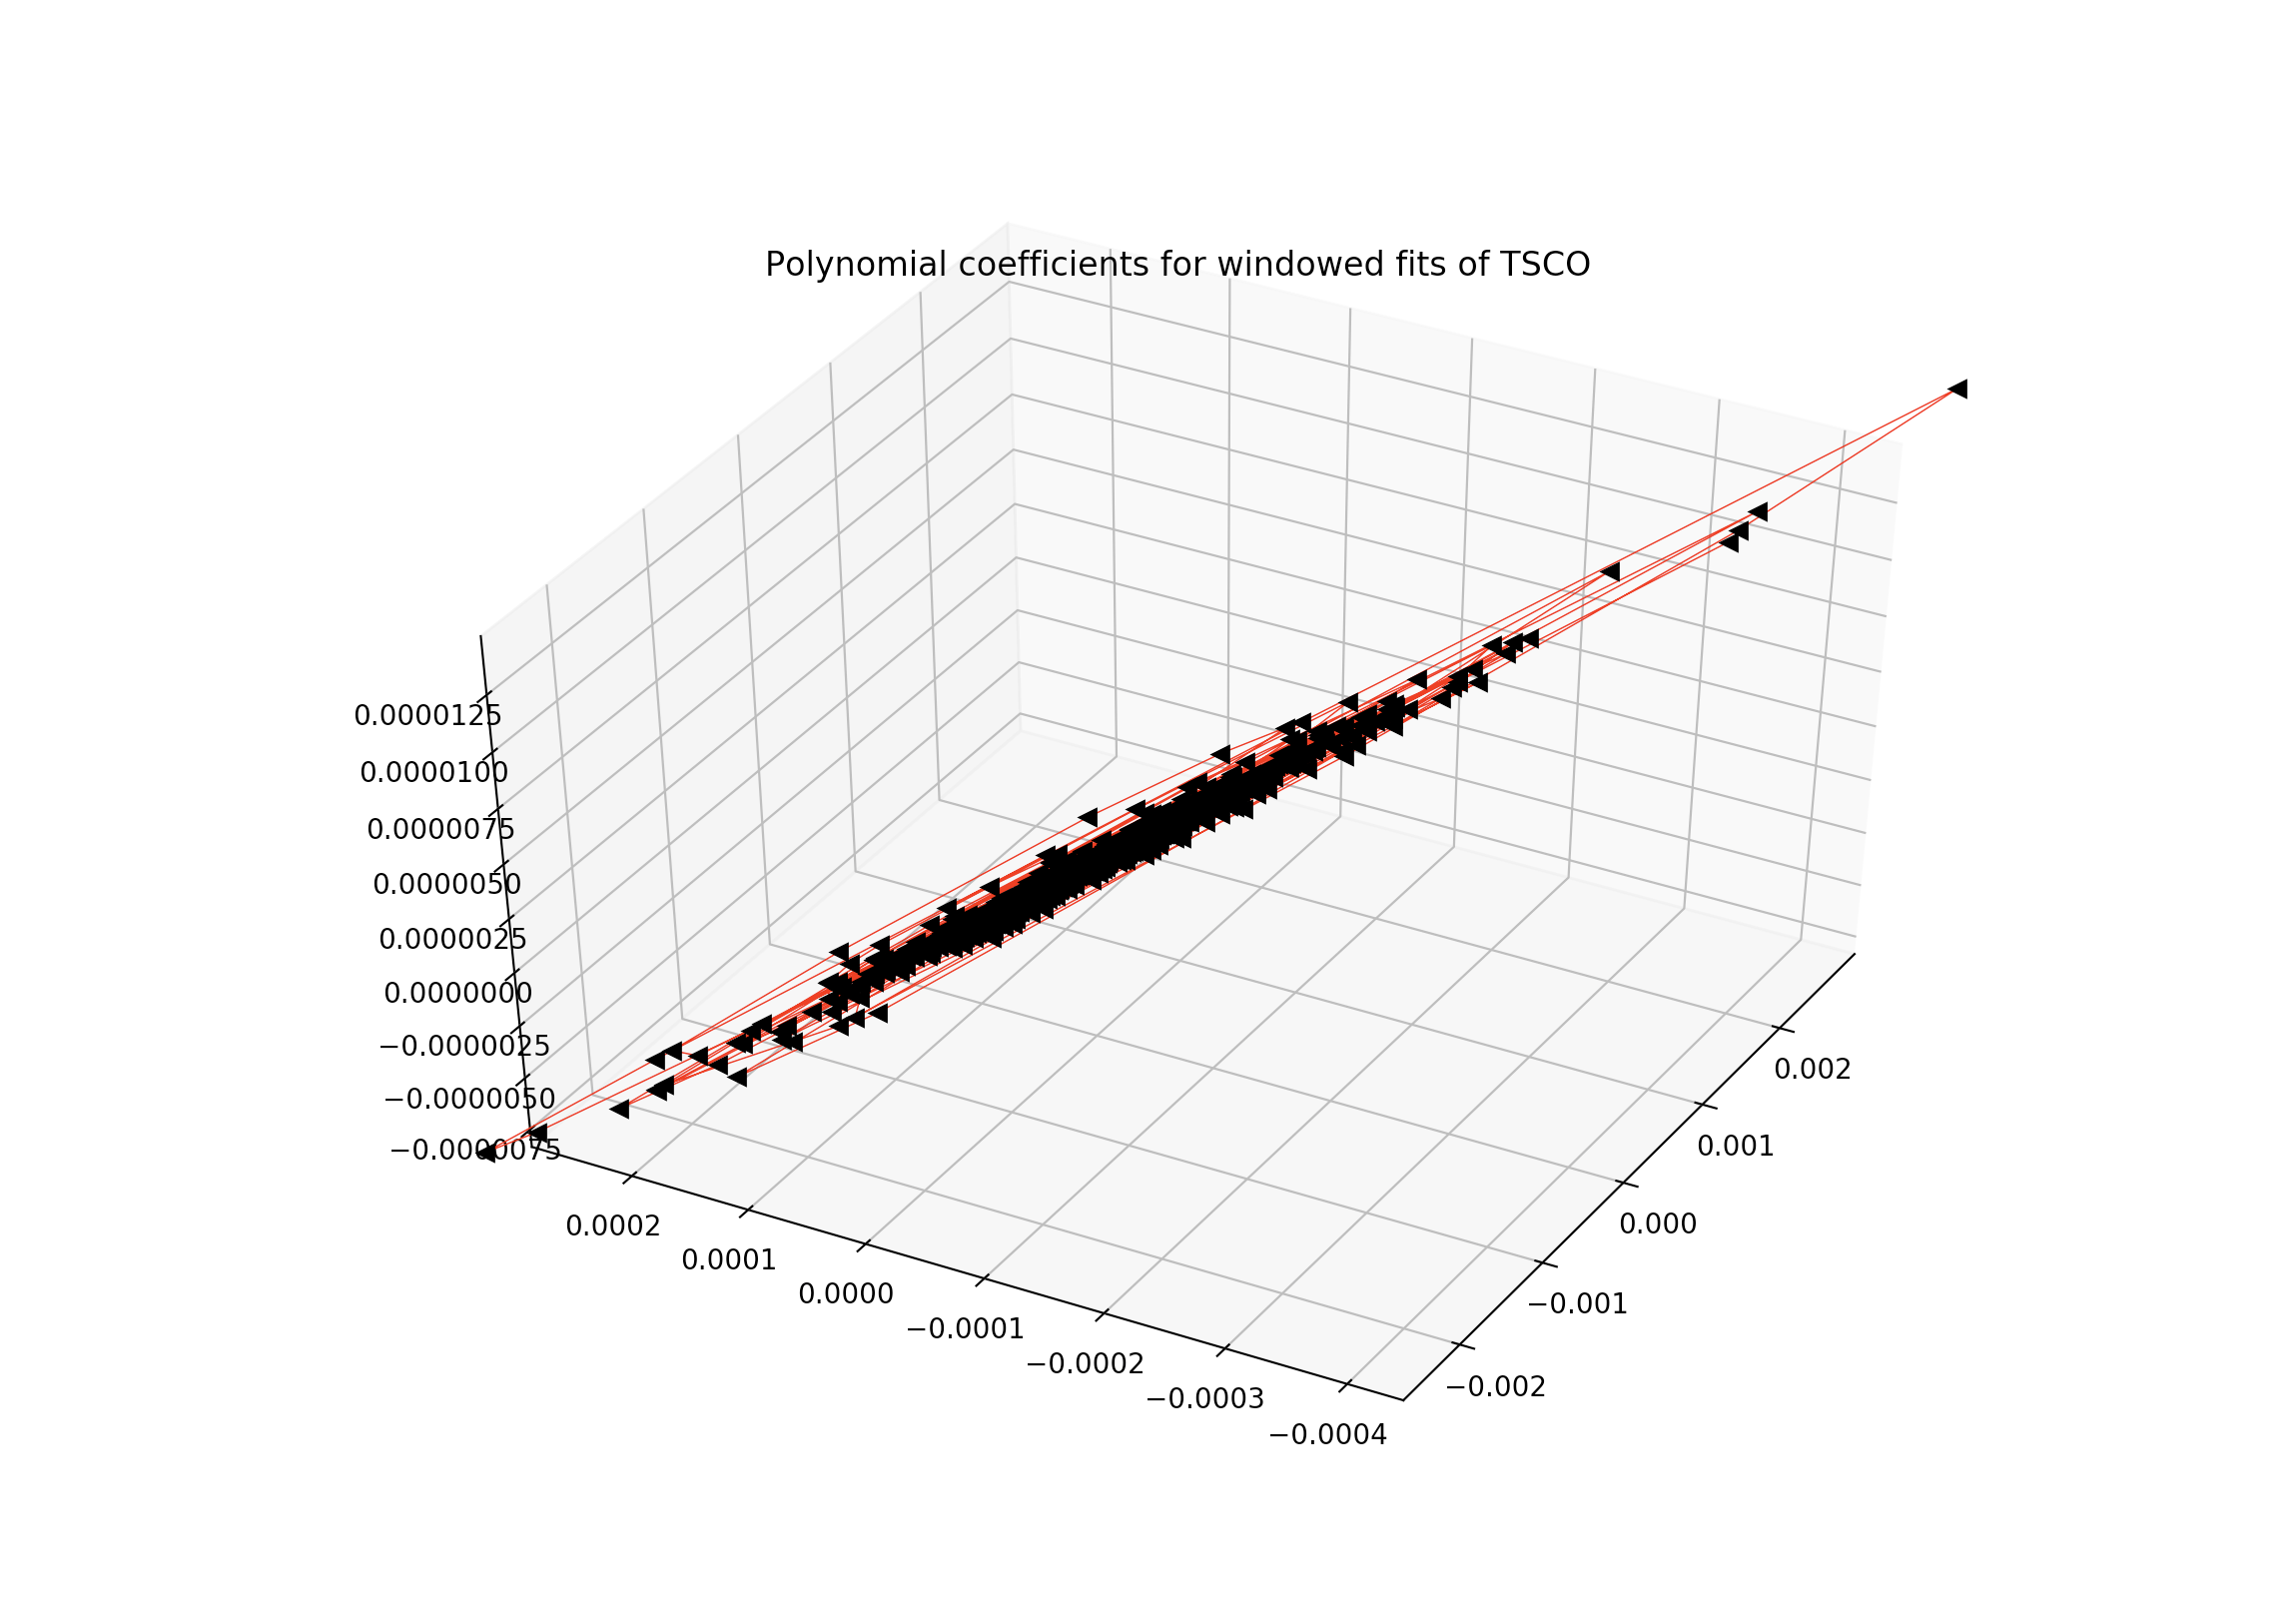
\includegraphics[width=\linewidth]{img/coeff2}
  \end{subfigure}
  \caption{Visualization of the lower order coefficients in $\mathbb{R}^3$}
  \label{fig:coeff}
\end{figure}

The distribution of the coefficients in three dimensional space seems to be a
multivariate Gaussian distribution. Furthermore, it seems to be very flat,
appearing to be a line if viewed from the correct angle. The trajectory of the
points also seems to be rotating around the center of the distribution.

\subsection{Frequency Analysis}


\end{document}
